\documentclass{article}
\usepackage{titlesec}
\usepackage{titletoc}
\usepackage{geometry}
\usepackage{enumitem}
\usepackage{setspace}
\usepackage{amsmath}
\usepackage{listings}
\usepackage{setspace}
\usepackage{graphicx}
\usepackage{float}
\usepackage{caption}
\usepackage{hyperref}
\usepackage{fancyhdr}

\date{}
\begin{document}
\begin{doublespace}
\title{\textbf{\vspace{1em}{}}}
\maketitle

\centering
{\LARGE \bfseries Computer Science 2XC3 - Final Project}
\vspace{3em}

{\Large Due Date: April 9, 2025 WINTER}\vspace{1.5em}

{\large \textbf{Group 9}}

{\large  Wu, Peter: \texttt{wu729}~\\
  Ganesh, Vikram: \texttt{vikramgv}~\\
  \vspace{0.5em}
  Bai, Franklin: \texttt{baif4}}~\\


\end{doublespace}

\newpage

\begin{onehalfspace}

\tableofcontents
\addcontentsline{toc}{section}{\large\normalfont {Part 1, Team Charter}}
\addcontentsline{toc}{section}{\large\normalfont {Part 2, Single Source Shortest Path Algorithms }}
\addcontentsline{toc}{section}{\large\normalfont {Part 3, All-pair Shortest Path Algorithm}}
\addcontentsline{toc}{section}{\large\normalfont {Part 4, A* Algorithm} }
\addcontentsline{toc}{section}{\large\normalfont {Part 5, Compare Shortest Path Algorithms}}
\addcontentsline{toc}{section}{\large\normalfont {Part 6, Organize code per UML Diagram} }~\\
\newpage


\section*{Part 1, Team Charter}
\subsection*{Communication}
\large{For our group, we decided that communication over \textbf{Discord} would be the most convenient for all members. Discord also allows screen sharing, making it a valuable tool for collaboration. Each member is expected to respond within \textbf{one hour} to maintain efficiency and work within our given timeframe.

For planned video calls, members are expected to join within \textbf{15 minutes} of the scheduled time. Since these meetings take up a significant portion of our schedules, punctuality is appreciated. If a member is unable to join, they must notify the group beforehand so the rest can plan accordingly. Any health or family emergencies will, of course, be waivered.

\textbf{Repeated failure} to adhere to the above communication agreements will result in an email to a TA or the professor, outlining the member's inability to meet agreed timeframes. This may lead to a deduction in their grade.

\subsection*{Collaboration Tools}

Our team will use \textbf{GitHub} to maintain version control. Each member may use the IDE of their choice, provided it is properly synced with Git. A shared repository will be created to store all code, diagrams, and other essential resources. This allows us to collaborate simultaneously, monitor each other's progress, and assist remotely.

The final report will be written using \textbf{LateX} to take advantage of its formatting capabilities compared to other programs. Sections may be drafted in other software and later copied or converted into LateX.

\subsection*{Dispute Resolution}

Team disputes will be resolved via a discussion on Discord or through a scheduled video call. During this discussion, the team will review the reasons behind any disagreements. If necessary, a second chance may be offered. 

If disputes cannot be resolved within the team and repeated failures occur, the matter will be escalated to a TA or the professor via email.

\subsection*{Deadlines and Task Allocation}

Our first internal deadline is \textbf{March 27th}, during which we will have a video call to discuss our progress on individual components of the project. We will have another internal deadline around \textbf{April 7th}, 2 days before the deadline, where we will begin finalizing our project.

Initial task distribution is as follows:

\begin{itemize}[leftmargin=1.5cm]
    \item \textbf{Franklin:} Part 1, 6
    \item \textbf{Vik:} Part 2, 3
    \item \textbf{Peter:} Part 4, 5
    \item \textbf{Team:} Part 7
\end{itemize}

These assignments are not final. Members are encouraged to assist one another, as we recognize the difficulty level may vary between different parts of the project.}
\newpage

\section*{Part 2}
In section 2, the modified versions of the dijkstra and bellman ford algorithms are implemented, where each algorithm was allowed to perform at most $k$ relaxations per node. Each implementation
was then tested and compared against the original versions of the algorithms for accuracy, performance and memory usage. The results of the tests are shown in the tables below.

\subsection*{Accuracy}

To measure the accuracy of the modified algorithms, we designed various experiments to determine how the size of the graph, density of the graph, and the number of relaxations per node (k value) 
affected the accuracy of the algorithms. The results of these experiments are shown in the graphs below. 
\smallskip
\newline
\indent The first experiment was designed to measure the accuracy of the modified algorithms with different k values. 
The results of this experiment are shown in Figure \ref{fig:Figure 1}.


\begin{figure}[H]
    \centering
    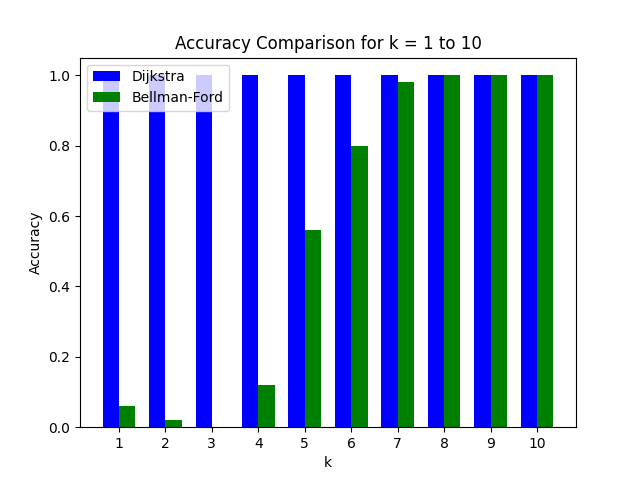
\includegraphics[width=0.8\textwidth]{Figures/Accuracy_kvals.png} 
    \caption{\footnotesize Experiment 1 - Accuracy of modified algorithms with different k values.}
    \label{fig:Figure 1} 
\end{figure}

This experiment was performed across 50 trials, where each trial consisted of a graph with 100 nodes, 200 edges and a maximum weight of 10. 
The results of this experiment show that the accuracy of the modified Bellman-Ford algorithm increases as the k value increases. This is because the modified Bellman-Ford algortihm is allowed to perform at most k relaxations per node, which means that they may not be able to find the shortest path in the graph if the k value is too small.
\smallskip
\newline
\indent However, the value of k does not seem to have any effect on the accuracy of the modified Dijkstra's algorithm, and the modified Dijkstra's algorithm is able to find the shortest path in the graph regardless of the value of k. This is because the modified Dijkstra's algorithm is able to find the shortest path in the graph by using a priority queue to keep track of the nodes that have been visited and the nodes that have not been visited.
Therefore, the value of k does not affect the accuracy of the modified Dijkstra's algorithm.
\smallskip
\newline

\indent The second and third experiments were designed to measure the accuracy of the modified algorithms with different graph sizes and densities. The results of these experiments are shown in Figure \ref{fig:Figure 2} and Figure \ref{fig:Figure 3}.

\begin{figure}[H] 
    \centering
    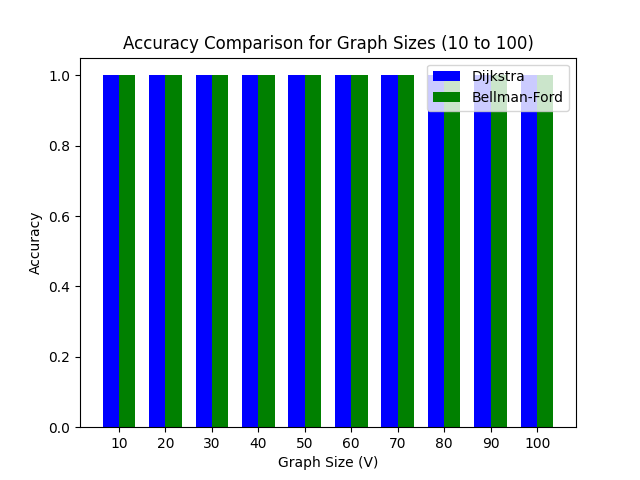
\includegraphics[width=0.7\textwidth]{Figures/Accuracy_sizes.png} 
    \caption{\footnotesize Experiment 2 - Accuracy of modified algorithms with different graph sizes.}
    \label{fig:Figure 2} 
\end{figure}

\begin{figure}[H] 
    \centering
    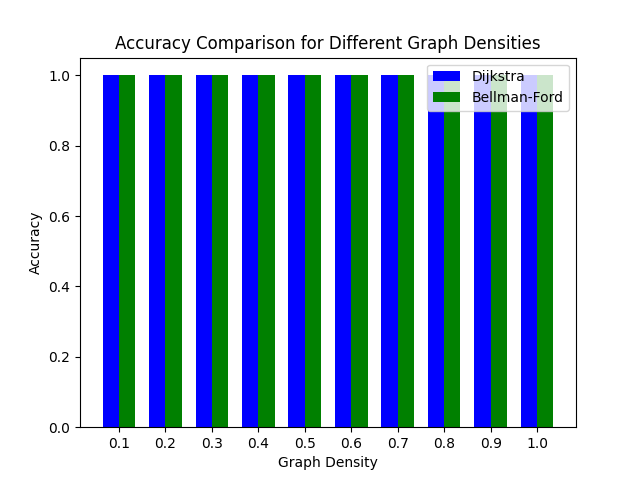
\includegraphics[width=0.7\textwidth]{Figures/Accuracies_densities.png} 
    \caption{\footnotesize Experiment 3 - Accuracy of modified algorithms with different graph densities.}
    \label{fig:Figure 3} 
\end{figure}

Experiment 2 was performed across 50 trials, where each trial consisted of a graph with $k=10$, a maximum edge weight of 10 and a density $D$ of 0.5. The experiment was conducted with $|V| = 10, ... , 100$ The number of vertices were calculated based on the number of edges in the graph using the following formula: $$\frac{|E| = |V|(|V| - 1) 0.5}{2}$$
where $|E|$ is the number of edges, $|V|$ is the number of vertices and $D$ is the density of the graph. 
\smallskip
\newline
\indent
Experiment 3 was performed across 50 trials, where each trial consisted of a graph with $k = 10$, a maximum edge weight of 10 and 20 vertices. The experiment was conducted with $D = 0.1, 0.2, ... , 1.0$. The density of the graph was calculated based on the number of edges in the graph using the following formula: $$\frac{|E| = 20(20 - 1) D}{2}$$
where $|E|$ is the number of edges, $|V|$ is the number of vertices and $D$ is the density of the graph.
\smallskip
\newline
\indent
The results of these experiments show that the accuracy of the modified Bellman-Ford and dijkstra's algorithms are not affected by the size of the graph
or the density of the graph. We can see this in Figure \ref{fig:Figure 2} and Figure \ref{fig:Figure 3}, where the accuracy of the modified Bellman-Ford and dijkstra's algorithms are 100\% for all graph sizes and densities. 
\smallskip
\newline
\indent
The results of these experiments show that the accuracy of the modified Bellman-Ford and dijkstra's algorithms are not affected by the size of the graph or the density of the graph, but Bellman-ford alone is 
affected by the number of relaxations allowed per node.

\subsection*{Time Complexity}
To measure the time complexity/performance of the modified algorithms, we designed various experiments
to determine how the size of the graphs, density of the graphs, and the number of relaxations per node (k value) affected the performance of the algorithms.
The results of these experiments are shown below.

Experiment 4 was designed to measure the performance of the modified algorithms with different $k$ values.
This experiment was conducted with the same parameters as 
experiment 1, where each trial consisted of a graph with 100 nodes, 200 edges, a maximum edge weight of 10 and $k$ values of $1, ... , 10$.
The results of this experiment are shown in Figure \ref{fig:Figure 4}. 
\begin{figure}[H] 
    \centering
    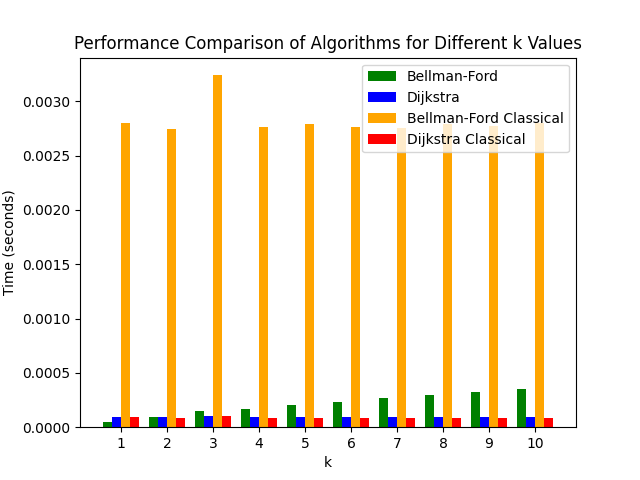
\includegraphics[width=0.7\textwidth]{Figures/Performance_kvals.png} 
    \caption{\footnotesize Experiment 4 - Performance of modified algorithms with different k values.}
    \label{fig:Figure 4} 
\end{figure}

The results of this experiment varied for each algorithm. The modified Bellman-Ford algorithm was significantly faster
than the original Bellman-Ford algorithm. However, the speed of the modified Bellman-Ford algorithm did increase as the value of $k$ increased, with more of 
a linear increase. This shows that restricting the number of relaxations per node allows the Bellman-Ford algorithm to perform significantly faster. Furthermore, the modified dijkstra's algorithm performed almost identically to the original dijkstra's algorithm, showing that the modified dijkstra's algorithm is not affected by the value of $k$.
Both versions of djikstra's algorithm performed faster than both versions of the Bellman-Ford algorithm, which is expected as dijkstra's algorithm is more efficient and has a better time complexity than Bellman-Ford ($O(E + V \log V)$ vs $O(VE)$).
\smallskip
\newline
\indent
Experiment 5 was designed to measure the performance of the modified algorithms with different graph sizes.
This experiment was conducted with the same parameters as experiment 2, where each trial consisted of a graph with $k=10$, a maximum edge weight of 10 and a density $D$ of 0.5. The number of vertices were calculated based on the number of edges in the graph using the same formula as experiment 2.
The results of this experiment are shown in Figure \ref{fig:Figure 5}.

\begin{figure}[H] 
    \centering
    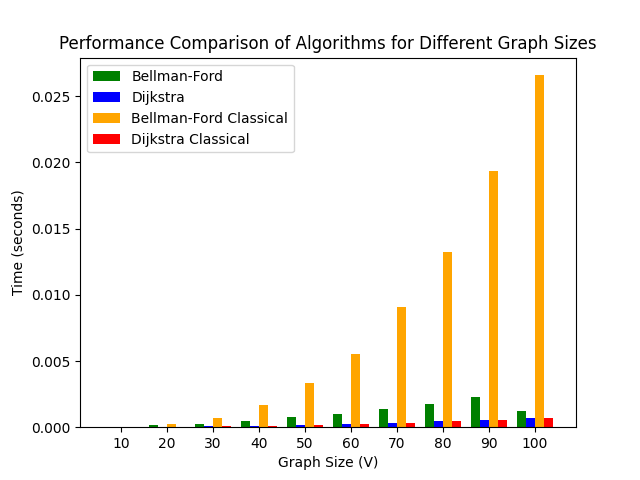
\includegraphics[width=0.7\textwidth]{Figures/Performance_sizes.png} 
    \caption{\footnotesize Experiment 5 - Performance of modified algorithms with different graph sizes.}
    \label{fig:Figure 5} 
\end{figure}

Here, the results are similar to experiment 4, with the excpetion of the classical Bellman-Ford algorithm's performance.
Both versions of bellman ford increased in time complexity as the number of vertices increased, with the classic Bellman-Ford algorithm decreasing in performance at a much faster rate
than the modified Bellman-Ford algorithm. This is because the modified Bellman-Ford algorithm is able to perform at most k relaxations per node, which means that it is able to perform faster than the classical Bellman-Ford algorithm.
Both version of djikstra's algorithm saw a decrease in performance as the numebr of vertices increased, but oth performed faster than each 
version of Bellman-Ford. The modified djikstra's algorithm performed very similarly to the classical dijkstra's algorithm, which is expected as the modified dijkstra's algorithm is not affected by the value of k.
This is to be expected, since djikstra's algorithm is more efficient and has a better time complexity than Bellman-Ford ($O(E + V \log V)$ vs $O(VE)$).
\smallskip
\newline
\indent
Experiment 6 was designed to measure the performance of the modified algorithms with different graph densities. 
It was conducted with the same parameters as experiment 3, where each trial consisted of a graph with $k=10$, a maximum edge weight of 10 and 20 vertices. The density of the graph was calculated based on the number of edges in the graph using the same formula as experiment 3.
The results of this experiment are shown in Figure \ref{fig:Figure 6}.

\begin{figure}[H] 
    \centering
    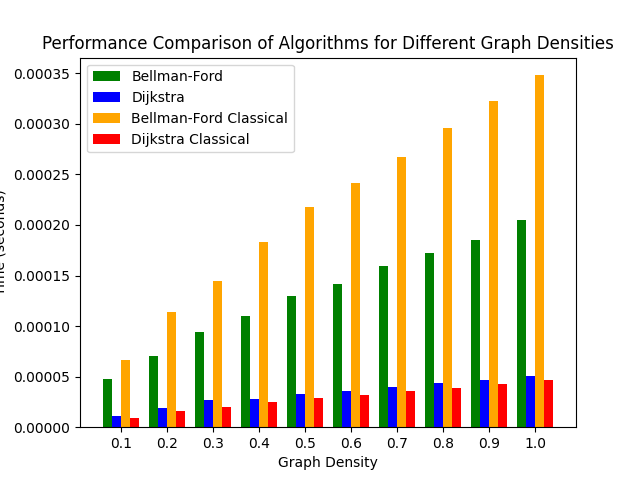
\includegraphics[width=0.7\textwidth]{Figures/Performance_densities.png} 
    \caption{\footnotesize Experiment 6 - Performance of modified algorithms with different graph densities.}
    \label{fig:Figure 6} 
\end{figure}

\newpage

Here, we can see that the density of the graph affects the performance of all the algorithms in a similar way.
Both versions of Bellman-Ford and dijkstra's algorithms saw a decrease in performance as the density of the graph increased, with the classical Bellman-Ford algorithm decreasing in performance at a much faster rate than the modified Bellman-Ford algorithm.
Similar to experiment 5, this is because the restriction of k relaxations per node allows the modified Bellman-Ford algorithm to perform faster than the classical Bellman-Ford algorithm.
The modified dijkstra's algorithm also performed similarly to the classical dijkstra's algorithm,
however, the modified dijkstra's algorithm performed slightly slower than the classical dijkstra's algorithm. however, the difference in perfoance was very small. 
Both of these algorithms performed faster than both versions of Bellman-Ford, which is expected as dijkstra's algorithm is more efficient and has a better time complexity than Bellman-Ford.
\smallskip
\newline
indent
Therefore, we can see that each parameter has different effects on the performance tiem of each algorithm.

\subsection*{Memory Usage}
Similar to the previous experiments, to calculate the memory usage of the modified algorithms, we designed various experiments to determine how the size of the graphs, density of the graphs, and the number of relaxations per node (k value) affected the memory usage of the algorithms.
\smallskip
\newline
\indent
Experiment 7 has designed to measure the memory usage of the modified algorithms with different $k$ values. The 
parameters of the experiment were the same as experimetn 1 and experiment 4, where each trial consisted of a graph with 100 nodes, 200 edges, a maximum edge weight of 10 and $k$ values of $1, ... , 10$.
The results of this experiment are shown in Figure \ref{fig:Figure 7}.

\begin{figure}[H] 
    \centering
    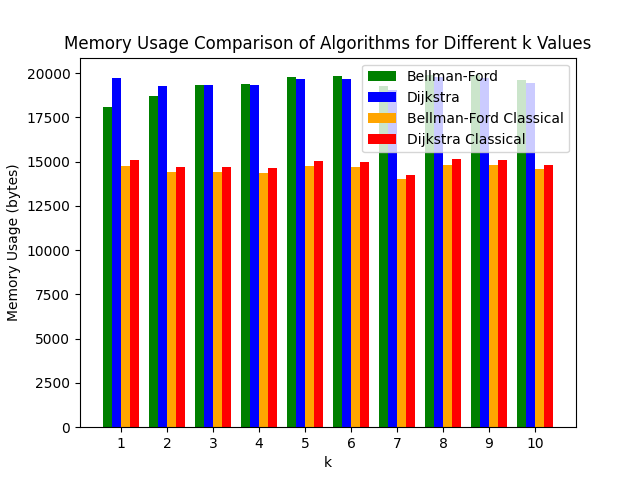
\includegraphics[width=0.8\textwidth]{Figures/Memory_kvals.png} 
    \caption{\footnotesize Experiment 7 - Memory usage of modified algorithms with different k values.}
    \label{fig:Figure 7} 
\end{figure}

Experiment 7 shows that the memory usage of every algorithm does not seem to be affected by the value of k, as the 
memory usage of each algorithm is relatively the same for all values of k. This is expected as the memory usage of each algorithm is determined by the number of vertices and edges in the graph, rather than the value of k.
Both the modified version of the Bellman-Ford algorithm and the modified version of dijkstra's algorithm used very similar amounts of memory as the classical versions of the algorithms.
Both of the modified algorithms also use more memory than the classical versions of the algorithms,
which is expected as the modified algorithms are more complex and have more variables to store and modify.
\smallskip
\newline
\indent

Therefore, we can see that the memory usage of each algorithmn is only affected by the number of vertices, and the density and size of the graph do not affect the memory usage of each algorithm.

Experiment 8 was designed to measure the memory usage of the modified algorithms with different graph sizes. The parameters of the experiment were the same as experiment 2 and experiment 5, where each trial consisted of a graph with $k=10$, a maximum edge weight of 10 and a density $D$ of 0.5. The number of vertices were calculated based on the number of edges in the graph using the same formula as experiment 2.
The results of this experiment are shown in Figure \ref{fig:Figure 8}.

\begin{figure}[H] 
    \centering
    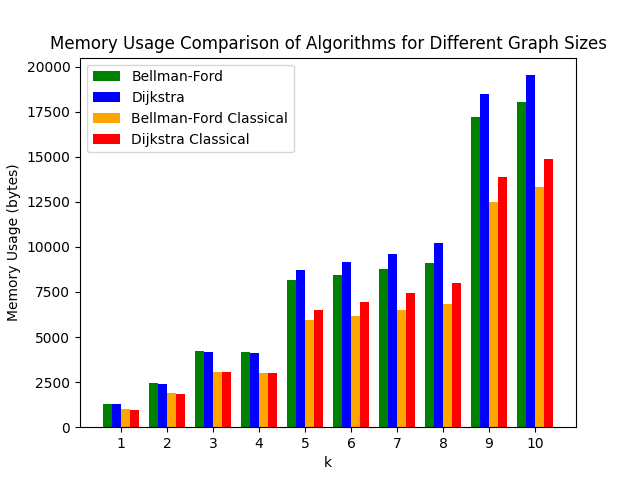
\includegraphics[width=0.8\textwidth]{Figures/Memory_sizes.png} 
    \caption{\footnotesize Experiment 8 - Memory usage of modified algorithms with different graph sizes.}
    \label{fig:Figure 8} 
\end{figure}

Experiment 8 shows that the memory usage of each algorithm increases as the number of vertices
in the graph increases. The classical versions of both algorithms perform faster than the modified
versions of the algorithms and use less memory than the modified versions of the algorithms. 
However, there is a clear trend among all algorithms, where the memory usage of each algorithm
increases as the number of vertices in the graph increases. This is expected as the number of vertices in the graph increases, as we know that the space complexity of both algorithms is $O(V)$, where $V$ is the number of vertices in the graph.
\smallskip
\newline
\indent
Experiment 9 was designed to measure the memory usage of the modified algorithms with different graph densities. 
The parameters of the experiment were the same as experiment 3 and experiment 6, where each trial consisted of a graph with $k=10$, a maximum edge weight of 10 and 20 vertices. The density of the graph was calculated based on the number of edges in the graph using the same formula as experiment 3.
The results of this experiment are shown in Figure \ref{fig:Figure 9}.

\begin{figure}[H] 
    \centering
    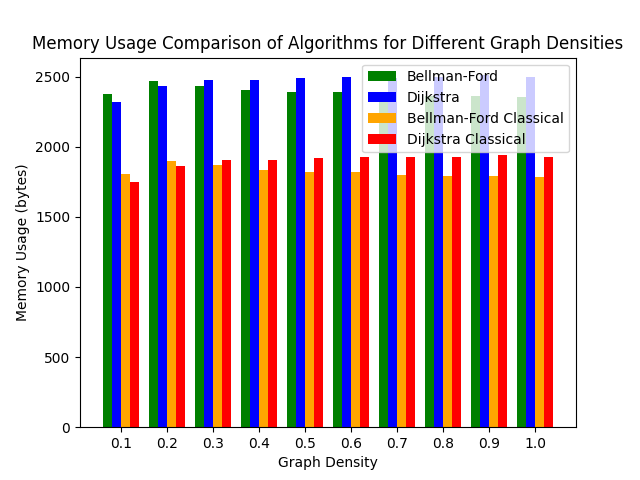
\includegraphics[width=0.8\textwidth]{Figures/Memory_densities.png} 
    \caption{\footnotesize Experiment 9 - Memory usage of modified algorithms with different graph sizes.}
    \label{fig:Figure 9} 
\end{figure}

Experiment 9 shows that the memory usage of each algorithm is not affected by the density of the graph, as the memory usage of each algorithm is relatively the same for all values of density.
This is expected as the memory usage of each algorithm is determined by the number of vertices and edges in the graph, rather than the density of the graph.
Hence, the results of this experiment are very similar to the reulsts of experiment 7, where both the modified version of the Bellman-Ford algorithm and the modified version of dijkstra's algorithm used very similar amounts of memory as the classical versions of the algorithms.

\section*{Part 3}
In section 3, an algorithm to find the shortest path in a graph from all nodes to a single node were implemented. 
This was implemented in two different ways, one using dijkstra's algorithm and the other using bellman ford.

\smallskip
For dense graphs, the single-source implementation of dijkstra's algorithm has a time complexity of $O(V^2)$,
where $V$ is the number of vertices in the graph, while it's time complexity for sparse graphs is $O(E + V \log V)$, where $E$ is the number of edges in the graph.
The implementation of the shortest path algorithm (for all nodes) using dijkstras has a time complexity of 
$O(V^3)$ for dense graphs and $O(E^2 + EV^2 \log V)$. This is because dijkstra's algorithm is run $V$ times, once for each node in the graph.

\smallskip
The same logic applies to the implementation of the shortest path algorithm using bellman ford. The time complexity for dense graphs is $O(V^3)$ and for sparse graphs is $O(E^2 + EV^2)$.
The implementation of the shortest path algorithm using bellman ford has a time complexity of $O(V^4)$ for dense graphs and $O(E^2 + EV^2)$ for sparse graphs. This is because bellman ford is run $V$ times, once for each node in the graph.


\section*{Part 4, A* Algorithm}
\newpage

\section*{Part 5, Compare Shortest Path Algorithms}
\newpage

\section*{Part 6, Organize code per UML Diagram}

The design principles and patterns being used in this diagram include composition, class inheritance, and adapters. 

HeuristicGraph inherits from WeightedGraph, which inherits from Graph class.

Dijkstras, Bellman\_Ford, and A\_star (which is an adapter class for original A\_star algorithm, another design principle) all inherit from SPAlgorithm.

Finally, ShortPathFinder uses composition (has-a relation) by passing a Graph object and interchangeable SPAlgorithm types into the class to help run. This way we can allow runtime switching of algorithms to whichever may be more efficient for the situation, especially using the set\_algorithm function.

Currently, nodes are represented as only integers which is very limiting in that it cannot represent much information. Thus, a solution could be implementing a custom Node class, where we can define metadata for each node, like name, value, date, or something similar. A sample implementation could be:

\begin{lstlisting}[language=Python]
class Node:
    def __init__(self, name: str, value: int, date: int):
        self.name = name
        self.value = value
        self.date = date

    def __repr__(self):
        return f"Node(name={self.name!r},
        value={self.value},date={self.date})"
\end{lstlisting}

Now whenever we need a node, we can pass in this Node object, which contains a lot more data than just a simple integer value.

This means we must change all classes that utilize nodes. We can change adjacency list from \texttt{List[int]} to \texttt{Dict[Node, List[Node]]}, or change weights to use \texttt{Dict[Tuple[Node, Node], float]}. Other sample changes include changing \texttt{add\_node(node: int)} function, to \texttt{add\_node(node: Node)}. And when we need specific values from Node, we can simply call \texttt{Node.name} or \texttt{Node.date}, etc. This would be a much better design for this UML.
%\section*{List of Figures}
%\startlist{toc}
%\printlist{toc}{section}{\textbf{Part 5, werlkwerjoik}}

\end{onehalfspace}
\end{document}
